\documentclass{article}
\usepackage{ctex}
\usepackage{geometry}
\usepackage{cite}
\usepackage{tikz}
\usepackage{xcolor}
\usepackage{listings}
\usepackage{graphicx}
\usetikzlibrary{graphs, positioning, quotes, shapes.geometric}
\usepackage{url}
\usepackage{threeparttable}
\usepackage{CJK}
\usepackage[colorlinks,
linkcolor=blue,
anchorcolor=blue, 
citecolor=blue,        
]{hyperref}
%\ctexset{bibname=}
\begin{document}
	\title{\vspace{+10pt} \heiti \textbf {智能水务分析模型}}
	\songti
	\author{}
	\date{}
	\maketitle  
	\section*{\centering \textbf{摘要}}
	q \cite{NBS}
	\newpage
	\section{问题重述}
		\subsection{问题背景}
			hehe \cite{kaldor1957model}
			\begin{figure}[htb]
			\centering
			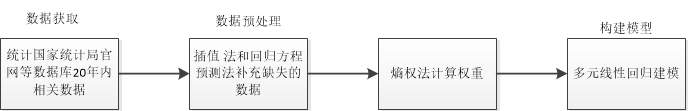
\includegraphics[width=10cm]{pictures/jmgc.png}
			\caption{建模过程}
			\label{jmgc}
			\end{figure}	
		aa\cite{ywf2017eduandeco}
		\subsection{需要解决的问题}
			hehe \cite[text]{sqf}
	\section{问题分析}	
		hehe
	\section{模型假设}
		anch
	\begin{itemize}
		\item 在经济建设中,主要由劳动人口作出贡献,因此用劳动人口数量和劳动人口的占比这两组变量来概括劳动人口规模
		\item 经济发展起点由前一年国内生产总值决定,资源禀赋由耕地面积和工业企业数量决定,教育水平由教育经费、教育的普及率、入学率和毕业生人数等决定
		\item 多重共线性检验后得到的模型,如果其在改进后依然存在严重的多重共线性,则进一步深入分析该模型,判断能不能忽略多重共线性对其的影响
		\item 该经济增长的回归模型是正确设定的
		\item 所有自变量的随机误差项满足正态分布且均值为0,且与相应自变量同方差、不序列相关
	\end{itemize}
	\section{模型主要变量符号及含义}
		\begin{center}
			\begin{threeparttable}
				\setlength{\tabcolsep}{10mm}
				\begin{tabular}{ccc}
				\hline
				序号 & 符号 & 意义\\
				\hline
				1 & Y1 & 国内生产总值\\
				2 & Y2 & 人均国内生产总值\\
				3 & Y3 & 人均国内生产总值增长率\\
				4 & X1 & 实际利用外商直接投资金额\\
				5 & X2 & 年度资源禀赋\\
				6 & X3 & 年度教育水平\\
				7 & X4 & 年度劳动人口规模\\
				8 & X5 & 该年经济发展起点\\
				9 & X6 & 虚拟变量A1\tnote{1}\\
				10 & X7 & 虚拟变量A2\tnote{2}\\
				11 & t & 年份\\
				\hline
				\end{tabular}
				\begin{tablenotes}
					\item [1] 当年无疫情影响经济增长
					\item [2] 当年有疫情影响经济增长
				\end{tablenotes}
			\end{threeparttable}
		\end{center}
		hehe
	\section{模型建立}
		a
	\section{模型的检验与修正}
		对
	\section{模型求解}
		dui
	\section{模型评价}
		hao
	\bibliographystyle{unsrt}
	\bibliography{refs.bib}
	\section*{附录}
	\subsection*{I 程序源代码}
		hehe
	\subsection*{II 支撑材料文件列表}
		hehe
	\begin{itemize}
		\item 分类原始数据.rar
		\item 原始数据汇总.xls
		\item 建模求解分析过程草稿.docx
		\item 数据处理过程,结果及代码.docx
	\end{itemize}
\end{document}